\documentclass[
	% -- opções da classe memoir --
	12pt,				% tamanho da fonte
	%openright,			% capítulos começam em pág ímpar (insere página vazia caso preciso)
	oneside,			% para impressão em recto e verso. Oposto a oneside
	a4paper,			% tamanho do papel.
	% -- opções da classe abntex2 --
	%chapter=TITLE,		% títulos de capítulos convertidos em letras maiúsculas
	%section=TITLE,		% títulos de seções convertidos em letras maiúsculas
	%subsection=TITLE,	% títulos de subseções convertidos em letras maiúsculas
	%subsubsection=TITLE,% títulos de subsubseções convertidos em letras maiúsculas
	% -- opções do pacote babel --
	english,			% idioma adicional para hifenização
	french,				% idioma adicional para hifenização
	spanish,			% idioma adicional para hifenização
	brazil				% o último idioma é o principal do documento
]{abntex2}

% ---
% Pacotes básicos
% ---
\usepackage{lmodern}			% Usa a fonte Latin Modern
\usepackage[T1]{fontenc}		% Selecao de codigos de fonte.
\usepackage[utf8]{inputenc}		% Codificacao do documento (conversão automática dos acentos)
\usepackage{lastpage}			% Usado pela Ficha catalográfica
\usepackage{indentfirst}		% Indenta o primeiro parágrafo de cada seção.
\usepackage{color}				% Controle das cores
\usepackage{graphicx}			% Inclusão de gráficos
\usepackage{float}
\usepackage{microtype} 			% para melhorias de justificação
\usepackage{multirow}           % para multiplas linhas em tabelas
% ---

% ---
% Pacotes de citações
% ---
\usepackage[brazilian,hyperpageref]{backref}	 % Paginas com as citações na bibl
\usepackage[alf]{abntex2cite}	% Citações padrão ABNT

% ---
% CONFIGURAÇÕES DE PACOTES
% ---

% ---
% Configurações do pacote backref
% Usado sem a opção hyperpageref de backref
\renewcommand{\backrefpagesname}{Citado na(s) página(s):~}
% Texto padrão antes do número das páginas
\renewcommand{\backref}{}
% Define os textos da citação
\renewcommand*{\backrefalt}[4]{
	\ifcase #1 %
		Nenhuma citação no texto.%
	\or
		Citado na página #2.%
	\else
		Citado #1 vezes nas páginas #2.%
	\fi}%
% ---

% ---
% Informações de dados para CcBraaAPA e FOLHA DE ROSTO
% ---
\titulo{Solus, um software para monitoramento de painéis solares}
\autor{Angelo Rodrigo Ribeiro da Silva\thanks{angelorodriigo.rs@gmail.com}}
\local{Boituva}
\data{2018, v-0.0.1}
\orientador{Dr. Marcelo Figueiredo Polido}
\instituicao{
  INSTITUTO FEDERAL DE EDUCAÇÃO, CIÊNCIA E TECNOLOGIA DE SÃO PAULO -- IFSP
  \par
  Curso de Análise e Desenvolvimento de Sistemas}
\tipotrabalho{Trabalho de conclusão de curso}
% O preambulo deve conter o tipo do trabalho, o objetivo,
% o nome da instituição e a área de concentração
\preambulo{Documentação para o software desenvolvido como trabalho de conclusão de curso para análise e desenvolvimento de sistemas no Instituto Federal de Educação, Ciência e Tecnologia de São Paulo, câmpus de Boituva.}
% ---

% ---
% Configurações de aparência do PDF final

% alterando o aspecto da cor azul
\definecolor{blue}{RGB}{41,5,195}

% informações do PDF
\makeatletter
\hypersetup{
     	%pagebackref=true,
		pdftitle={\@title},
		pdfauthor={\@author},
    	pdfsubject={\imprimirpreambulo},
	    pdfcreator={LaTeX with abnTeX2 and Compiled with Pdflatex},
		pdfkeywords={painel solar}{ifsp}{arduino},
		colorlinks=true,       		% false: boxed links; true: colored links
    	linkcolor=blue,          	% color of internal links
    	citecolor=blue,        		% color of links to bibliography
    	filecolor=magenta,      		% color of file links
		urlcolor=blue,
		bookmarksdepth=4
}
\makeatother
% ---

% ---
% Espaçamentos entre linhas e parágrafos
% ---

% O tamanho do parágrafo é dado por:
\setlength{\parindent}{1.3cm}

% Controle do espaçamento entre um parágrafo e outro:
\setlength{\parskip}{0.2cm}  % tente também \onelineskip

% ---
% compila o indice
% ---
\makeindex
% ---

% ----
% Início do documento
% ----
\begin{document}

% Seleciona o idioma do documento (conforme pacotes do babel)
\selectlanguage{brazil}

% Retira espaço extra obsoleto entre as frases.
\frenchspacing

% --------------------------------
% ELEMENTOS PRÉ-TEXTUAIS
% --------------------------------
% ---
% Capa
% ---
\imprimircapa
% ---

% ---
% Folha de rosto
% (o * indica que haverá a ficha bibliográfica)
% ---
\imprimirfolhaderosto*
% ---

%% ---
% Inserir a ficha bibliografica
% ---

% Isto é um exemplo de Ficha Catalográfica, ou ``Dados internacionais de
% catalogação-na-publicação''. Você pode utilizar este modelo como referência.
% Porém, provavelmente a biblioteca da sua universidade lhe fornecerá um PDF
% com a ficha catalográfica definitiva após a defesa do trabalho. Quando estiver
% com o documento, salve-o como PDF no diretório do seu projeto e substitua todo
% o conteúdo de implementação deste arquivo pelo comando abaixo:
%
% \begin{fichacatalografica}
%     \includepdf{fig_ficha_catalografica.pdf}
% \end{fichacatalografica}

\begin{fichacatalografica}
	\sffamily
	\vspace*{\fill}					% Posição vertical
	\begin{center}					% Minipage Centralizado
	\fbox{\begin{minipage}[c][8cm]{13.5cm}		% Largura
	\small
	\imprimirautor
	%Sobrenome, Nome do autor

	\hspace{0.5cm} \imprimirtitulo  / \imprimirautor. --
	\imprimirlocal, \imprimirdata-

	\hspace{0.5cm} \pageref{LastPage} p. : il. (algumas color.) ; 30 cm.\\

	\hspace{0.5cm} \imprimirorientadorRotulo~\imprimirorientador\\

	\hspace{0.5cm}
	\parbox[t]{\textwidth}{\imprimirtipotrabalho~--~\imprimirinstituicao,
	\imprimirdata.}\\

	\hspace{0.5cm}
		1. Palavra-chave1.
		2. Palavra-chave2.
		2. Palavra-chave3.
		I. Orientador.
		II. Universidade xxx.
		III. Faculdade de xxx.
		IV. Título
	\end{minipage}}
	\end{center}
\end{fichacatalografica}
% ---


%% ---
% Inserir errata
% ---
\begin{errata}

\vspace{\onelineskip}

FERRIGNO, C. R. A. \textbf{Tratamento de neoplasias ósseas apendiculares com
reimplantação de enxerto ósseo autólogo autoclavado associado ao plasma
rico em plaquetas}: estudo crítico na cirurgia de preservação de membro em
cães. 2011. 128 f. Tese (Livre-Docência) - Faculdade de Medicina Veterinária e
Zootecnia, Universidade de São Paulo, São Paulo, 2011.

\begin{table}[htb]
\center
\footnotesize
\begin{tabular}{|p{1.4cm}|p{1cm}|p{3cm}|p{3cm}|}
  \hline
   \textbf{Folha} & \textbf{Linha}  & \textbf{Onde se lê}  & \textbf{Leia-se}  \\
    \hline
    1 & 10 & auto-conclavo & autoconclavo\\
   \hline
\end{tabular}
\end{table}

\end{errata}
% ---


%% ---
% Inserir folha de aprovação
% ---

% Isto é um exemplo de Folha de aprovação, elemento obrigatório da NBR
% 14724/2011 (seção 4.2.1.3). Você pode utilizar este modelo até a aprovação
% do trabalho. Após isso, substitua todo o conteúdo deste arquivo por uma
% imagem da página assinada pela banca com o comando abaixo:
%
% \includepdf{folhadeaprovacao_final.pdf}
%
\begin{folhadeaprovacao}

  \begin{center}
    {\ABNTEXchapterfont\large\imprimirautor}

    \vspace*{\fill}\vspace*{\fill}
    \begin{center}
      \ABNTEXchapterfont\bfseries\Large\imprimirtitulo
    \end{center}
    \vspace*{\fill}

    \hspace{.45\textwidth}
    \begin{minipage}{.5\textwidth}
        \imprimirpreambulo
    \end{minipage}%
    \vspace*{\fill}
  \end{center}

  \begin{center}
   \imprimirlocal, 4 de dezembro de 2018
  \end{center}

  Banca examinadora:

  \begin{center}
    \noindent\rule{16cm}{0.4pt}
    \vspace{0.1mm}
    (Titulação, nome completo, instituição)

    \vspace{5mm}

    \noindent\rule{16cm}{0.4pt}
    \vspace{0.1mm}
    (Titulação, nome completo, instituição)

    \vspace{5mm}

    \noindent\rule{16cm}{0.4pt}
    \vspace{0.1mm}
    (Titulação, nome completo, instituição)
  \end{center}

\end{folhadeaprovacao}
% ---


%% ---
% Dedicatória
% ---
\begin{dedicatoria}
   \vspace*{\fill}
   \centering
   \noindent
   \textit{Lorem ipsum dolor sit amet, consectetur adipisicing elit, sed do eiusmod tempor incididunt ut labore et dolore magna aliqua. Ut enim ad minim veniam, quis nostrud exercitation ullamco laboris nisi ut aliquip ex ea commodo consequat.} \vspace*{\fill}
\end{dedicatoria}
% ---


%% ---
% Agradecimentos
% ---
\begin{agradecimentos}

Lorem ipsum dolor sit amet, consectetur adipisicing elit, sed do eiusmod tempor incididunt ut labore et dolore magna aliqua. Ut enim ad minim veniam, quis nostrud exercitation ullamco laboris nisi ut aliquip ex ea commodo consequat.

\end{agradecimentos}
% ---


%% ---
% Epígrafe
% ---
\begin{epigrafe}
    \vspace*{\fill}
	\begin{flushright}
		\textit{`Lorem ipsum dolor sit amet, consectetur adipisicing elit, sed do eiusmod tempor incididunt ut labore et dolore magna aliqua. Ut enim ad minim veniam, quis nostrud exercitation ullamco laboris nisi ut aliquip ex ea commodo consequat. Duis aute irure dolor in reprehenderit in voluptate velit esse cillum dolore eu fugiat nulla pariatur. Excepteur sint occaecat cupidatat non proident, sunt in culpa qui officia deserunt mollit anim id est laborum.`}
	\end{flushright}
\end{epigrafe}
% ---


%% ---
% RESUMOS
% ---

% resumo em português
\setlength{\absparsep}{18pt} % ajusta o espaçamento dos parágrafos do resumo
\begin{resumo}
  A aplicação desenvolvida baseia-se na dificuldade durante a análise de dados meteorológicos perante a prévia instalação e configuração de painéis solares. Este documento visa documentar e descrever um software com foco na captura e análise de dados meteorológicos, produzindo assim, resultados e informações necessárias para o usuário.

 \textbf{Palavras-chave}: nodejs. painéis solares. energia solar. arduino.
\end{resumo}

% resumo em inglês
\begin{resumo}[Abstract]
 \begin{otherlanguage*}{english}
  The application developed is based on the difficulty during the analysis of meteorological data before the previous installation and configuration of solar panels. This document aims to document and describe a software focused on the capture and analysis of meteorological data, thus producing results and information necessary to the user.

   \vspace{\onelineskip}

   \noindent
   \textbf{Keywords}: nodejs. solar panels. solar energy. arduino.
 \end{otherlanguage*}
\end{resumo}


% ---
% inserir lista de ilustrações
% ---
\pdfbookmark[0]{\listfigurename}{lof}
\listoffigures*
\cleardoublepage
% ---

% ---
% inserir lista de tabelas
% ---
\pdfbookmark[0]{\listtablename}{lot}
\listoftables*
\cleardoublepage
% ---

% ---
% inserir lista de abreviaturas e siglas
% ---
\begin{siglas}
  \item{API} Application Programming Interface (em português Interface de Programação de Aplicações).
  \item{HTTP} HyperText Transfer Protocol (em português Protocolpo de transferência de hipertexto).
  \item{IFSP} Instituto Federal de Educação, Ciência e Tecnologia de São Paulo
  \item{RESTFUL API} Full Representational State Transfer Application Programming Interface (em português é um serviço de API que segue a risca as definições da abstração REST)
\end{siglas}
% ---


%% ---
% inserir lista de símbolos
% ---
\begin{simbolos}
\end{simbolos}
% ---


% ---
% inserir o sumario
% ---
\pdfbookmark[0]{\contentsname}{toc}
\tableofcontents*
\cleardoublepage
% ---


% --------------------------------
% ELEMENTOS TEXTUAIS
% --------------------------------
\textual

\nocite{ddd_eric_evans}
\nocite{gof_patterns}
\nocite{sonda_project}
\nocite{nosql_distilled}

% ----------------------------------------------------------
% Introdução (exemplo de capítulo sem numeração, mas presente no Sumário)
% ----------------------------------------------------------
\chapter{Introdução}
\addcontentsline{toc}{chapter}{Introdução}
% ----------------------------------------------------------

\section{Contextualização}

Na sociedade contemporânea, diversas preocupações quanto a captação de energia surgiram. Uma dessas preocupações é cada vez mais, buscar fontes renováveis de energia.

Atualmente, a energia solar vem mostrando seus benefícios, sendo pelo custo, que é mais baixo do que outras soluções e pela facilidade de instalação, que pode ser feita sem a necessidade de uma grande área reservada.

Devido ao avanço da captação de energia solar, desafios surgiram ao se estudar a melhor forma de se trabalhar com a energia captada.

\section{Tema}

O mote acerca do desenvolvimento desse trabalho, gira entorno do auxílio da tomada de decisão através do desenvolvimento de um software de análise e visualização de dados.

\section{Objetivo}

Este desenvolvimento tem como objetivo introduzir a questão da análise de dados meteorológicos e tomada de decisão acerca da instalação de painéis solares e documentar através de metodologias de descrição de software, a arquitetura e desenvolvimento de uma aplicação que visa auxiliar na resolução deste problema.

\section{Delimitação do Problema}

Não existe hoje uma forma prática, de baixo custo e precisa de realizar a análise de dados ante a instalação de painéis solares, visando, com uma massa de dados dispostos de maneira simples e organizada, auxiliar a tomada de decisão na instalação destes painéis, procurando através de variáveis como posição, ângulo entre outras, extrair o máximo de performance na captação de energia solar.

\section{Justificativa}

Existe um projeto de instalação de uma usina solar no IFSP, no campus localizado em Boituva, portanto, o tema do projeto foi escolhido, para que se possa através da análise prévia de dados, se encontrar a melhor configuração para os painéis fotovoltaicos, atingindo assim, uma maior captação de energia e aproveitamento de investimento.

\section{Método}

A metodologia de trabalho escolhida para este projeto, utiliza algumas convenções da metologia SCRUM, porém, pelo tamanho limitado da equipe, o projeto foi trabalhado sendo ditado pela metodologia KANBAN.
Para medirmos a qualidade do software, foi decidido optar pelo desenvolvimento da aplicação utilizando-se de técnicas de controle de qualidade orientadas ao teste.


\chapter{Descrição Geral do Sistema}
\addcontentsline{toc}{chapter}{Descrição Geral do Sistema}

O projeto visa, através da análise estatística de dados meteorológicos, auxiliar o estudo de viabilidade acerca da instalação de painéis fotovoltaicos.

Para isso, serão coletados dados através de sensores conectados a um microcontrolador arduino. Inicialmente, prevemos captar informações de umidade do ar, temperatura e incidência de radiação solar.

Dados esses, que serão enviados através de requisições HTTP para uma API, serão armazenadas em banco de dados e então, será feita uma análise estatística.

A interface do usuário final com a aplicação, será feita através de uma aplicação web, onde os dados analisados serão disponibilizados e o usuário fará consultas a essas informações.

\section{Descrição do Problema}

Durante o estudo de viabilidade sobre a instalação de painéis fotovoltaicos no IFSP, notou-se uma dificuldade na captura e análise dos dados para tomada de decisão, justificando assim, a necessidade da automatização desse processo, considerando também, a quantidade massiva de dados e as possíveis falhas de estimativa pelo cálculo humano.

Pelo alto de custo de instalação de painéis solares, uma decisão errada no estudo de viabilidade poderia causar um dano financeiro imensurável.

O sistema afeta principalmente, a configuração dos painéis como ângulo, posição, local, entre outras variaveis que podem afetar o desempenho energético.

\section{Principais Envolvidos e suas Características}

\subsection{Usuários do Sistema}

O sistema visa atender especialistas que precisam realizar tomadas de decisão.

Isso inclui também, clientes que, antes de realizar a instalação de painéis solares, precisam analisar se o investimento será compensado. E também, empresas de instalação de painéis solares, que gostariam de fazer uma análise de viabilidade mudando local, angulo e fazendo outras pesquisas acerca da instalação ou da manutenção de painéis fotovoltaicos.

\subsection{Desenvolvedores do Sistema}

Os envolvidos no desenvolvimento do projeto, são o orientador, Dr. Marcelo Polido, que ficará responsável pelos requisitos do sistema, ele irá coordenar o que será implementado e irá ditar as entregas incrementais. Também responsável por requisitos do projeto está o Professor Mario Pin, que será algo próximo de um Product Owner, ele será o primeiro cliente final da aplicação, irá utilizar o sistema para realizar análise de dados.

O planejamento e desenvolvimento do projeto, ficará por conta do aluno responsável pela defesa do mesmo, Angelo Silva.

O projeto é open source, ou seja, aberto para a comunidade no github, recebendo então, pequenas contribuições esporádicas de outros desenvolvedores ao longo do ciclo de vida do projeto.

\subsection{Tecnologias Empregadas}

A aplicação foi desenvolvida utilizando arduino para gerenciamento e captura dos dados utilizando requisições HTTP através das libraries do arduino. A conexão com a internet foi feita utilizando um arduino ethernet shield wifi, as informações são capturadas, é feita uma validação e formatação básica dos dados e então os mesmos são enviados para uma RESTFUL API construída com PHP.

A API do projeto foi desenvolvida utilizando microframework Lumen, utilizando banco de dados MYSQL e Percona server como SGBD, através de uma interface construída com framework front end bootstrap, javascript ES6 e sass, a interface foi construída seguindo conceitos de usabilidade.

\section{Regras de Negócio}

A maior parte das regras de negócio de sistema fica centralizada nos filtros, eles são quem valida os dados do sistema, definindo regras para a captura de dados.
A regra de negócio de filtragem diz que os dados de umidade e temperatura não podem se diferenciar por 50\% ou mais da média dos dados captados na ultima hora.


\chapter{Requisitos do sistema}
\addcontentsline{toc}{chapter}{Requisitos do sistema}

\section{Requisitos funcionais}

Os requisitos funcionais do sistema são definidos pelas características para que um MVP possa ser entregue.
Os requisitos são descritos no diagrama de caso de uso abaixo.

\begin{figure}[!htb]
    \label{figure_diagrama_caso_uso}
    \centering
    \caption{Diagrama de caso de uso} \label{includegraphics_diagrama_caso_uso}
    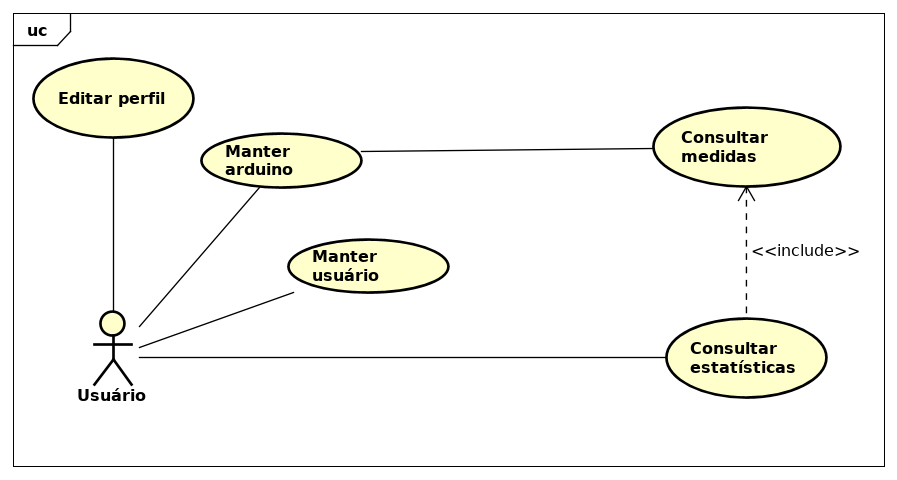
\includegraphics[scale=0.6]{diagrams/caso_de_uso.png}
    \hfill
\end{figure}

Os atores do sistema foram definidos com o o próprio sistema, que poderá realizar acesso a alguns casos de uso e o usuário final.
Seguem abaixo as especificações dos casos de uso.

\begin{table}
    \ABNTEXfontereduzida
    \caption{Especificações do caso de uso capturar dados meteorológicos}
    \label{my-label}
    \begin{tabular}{{l}|p{9.0cm}}

    \hline

    \multicolumn{2}{c}{\textbf{Capturar dados meteorológicos}} \\

    \hline
    Descrição & Captura os dados meteorológicos através de sensores conectados ao microcontrolador arduino e os envia através de requisição HTTP para a API \\

    \hline

    Atores & Sistema \\

    \hline

    \multirow{2}{*}{Pré-condições} & Credenciais de acesso a API \\
    & API em correto funcionamento \\

    \hline

    \multirow{2}{*}{Exceções e fluxos alternativos} & Em caso de perca de conexão com internet ou a API, armazena as informações temporariamente no Arduino \\

    \hline

    \end{tabular}
\end{table}

\begin{table}
    \ABNTEXfontereduzida
    \caption{Especificações do caso de uso armazenar dados meteorológicos}
    \label{my-label}
    \begin{tabular}{{l}|p{9.0cm}}

    \hline

    \multicolumn{2}{c}{\textbf{Armazenar dados meteorológicos}} \\

    \hline
    Descrição & Após receber os dados captados pelo arduino, a api os valida e então, os armazena em banco de dados \\

    \hline

    Atores & Sistema \\

    \hline

    \multirow{2}{*}{Pré-condições} & Banco de dados em correto funcionamento  \\
    & Recebimento de dados através das rotas da API \\

    \hline

    \multirow{2}{*}{Exceções e fluxos alternativos} & Em caso de dados inválidos, a API os descarta \\

    & Em caso de perca de conexão com banco de dados, a API os armazena em memória \\

    \hline

    \end{tabular}
\end{table}

\begin{table}
    \ABNTEXfontereduzida
    \caption{Especificações do caso de uso realizar consultas com filtros}
    \label{my-label}
    \begin{tabular}{{l}|p{9.0cm}}

    \hline

    \multicolumn{2}{c}{\textbf{Realizar consultas com filtros}} \\

    \hline
    Descrição & Recebe do usuário os filtros para seleção das informações, então, realiza uma análise estatística dos dados requeridos e os exibe para o usuário utilizando gráficos. \\

    \hline

    Atores & Usuário \\

    \hline

    \multirow{3}{*}{Pré-condições} & Credenciais de acesso ao banco de dados para realizar as consultas  \\
    & Banco de dados em correto funcionamento \\
    & Filtros corretos passados pelo usuário \\

    \hline

    \multirow{2}{*}{Exceções e fluxos alternativos} & Caso ele não encontre dados na seleção, exibe uma mensagem de não encontrado  \\

    & Em caso de perca de conexão com banco de dados, exibe uma tela de erro ao usuário \\

    \hline

    \end{tabular}
\end{table}

\begin{table}
    \ABNTEXfontereduzida
    \caption{Especificações do caso de uso realizar análise estatística dos dados}
    \label{my-label}
    \begin{tabular}{{l}|p{9.0cm}}

    \hline

    \multicolumn{2}{c}{\textbf{Realizar análise estatística dos dados}} \\

    \hline
    Descrição & Realiza calculo estatístico de informações, retornando informações relevantes como média, moda e desvio padrão. \\

    \hline

    Atores & Usuário \\

    \hline

    \multirow{2}{*}{Pré-condições} & Credenciais de acesso ao banco de dados  \\
    & Banco de dados em correto funcionamento \\

    \hline

    \multirow{2}{*}{Exceções e fluxos alternativos} & Caso não existam dados para serem analisados, joga uma exceção de argumentos inválidos  \\

    \end{tabular}
\end{table}

\section{Requisitos não funcionais}

Os requisitos não funcionais do sistema complementam os requisitos funcionais, como melhorias para as especificações.

\subsection{Segurança}

O projeto precisa trabalhar de forma segura, então, esse requisito pede para que a API possua autenticação das aplicações clientes e que também, a aplicação web possua autenticação, para o usuário visualizar as informações e realizar consultas, ele precisa estar autenticado.

\subsection{Disponibilidade}

Para garantir uma melhor análise e fidelidade dos dados, o sistema precisa funcionar durante 24 horas por dia e 7 dias por semana, para isso, redundâncias precisam ser trabalhadas.

\subsection{Performance}

Outro requisito não funcional do sistema é a performance, as informações precisam ser processadas de forma rápida, problemas como lentidão no processamento podem acabar acavalando a aplicação.


\chapter{Análise dos dados capturados}
\addcontentsline{toc}{chapter}{Análise dos dados capturados}

As informações que foram capturadas pelo microcontrolador, ao serem requisitadas pelo usuário, são disponibilizadas através de uma interface gráfica, utilizando análise de estatística e gráficos.

\section{Filtros}

Os filtros utilizados pelo usuário, são a estação meteorológica que ele deseja visualizar, a data inicial e a data final para busca dos dados e o intervalo para calculo das médias.

\subsection{Tratamento de dados}

Os dados foram exibidos da mesma forma que foram capturados, com exceção das informações de intensidade de luz, que foi invertida para melhor exibição no gráfico, e pela medida de nível de chuva, que além de invertida, foi transformada em porcentagem.

\section{Resultados}

\subsection{Médias}

A média aplicada em cima dos dados, é separada por um intervalo de tempo, como exemplo, caso o usuário informe que o intervalo requisitado é de uma hora, os dados são agrupados por cada hora e então, uma média é aplicada nesses dados, exibindo as médias em intervalos de horas no gráfico.

\subsection{Mínimas e Máximas}

É exibida também uma lista com as mínimas e máximas daquela estação meteorológica no intervalo de tempo informado.

\chapter{Diagrama de classes}
\addcontentsline{toc}{chapter}{Diagrama de classes}

Como podemos verificar no diagrama descrito na figura \ref{figure_diagrama_classe} as entidades do sistema consistem na medida, que é a informação que foi capturada pelo arduino, uma entidade abstrata que é entendida pelas classes concretas das medidas, temos também as entidades que representam o arduino, possuindo a localização do mesmo e o usuário, ambos extendendo da classe autentical.

\begin{figure}[H]
    \label{figure_diagrama_classe}
    \centering
    \caption{Diagrama de classes}
    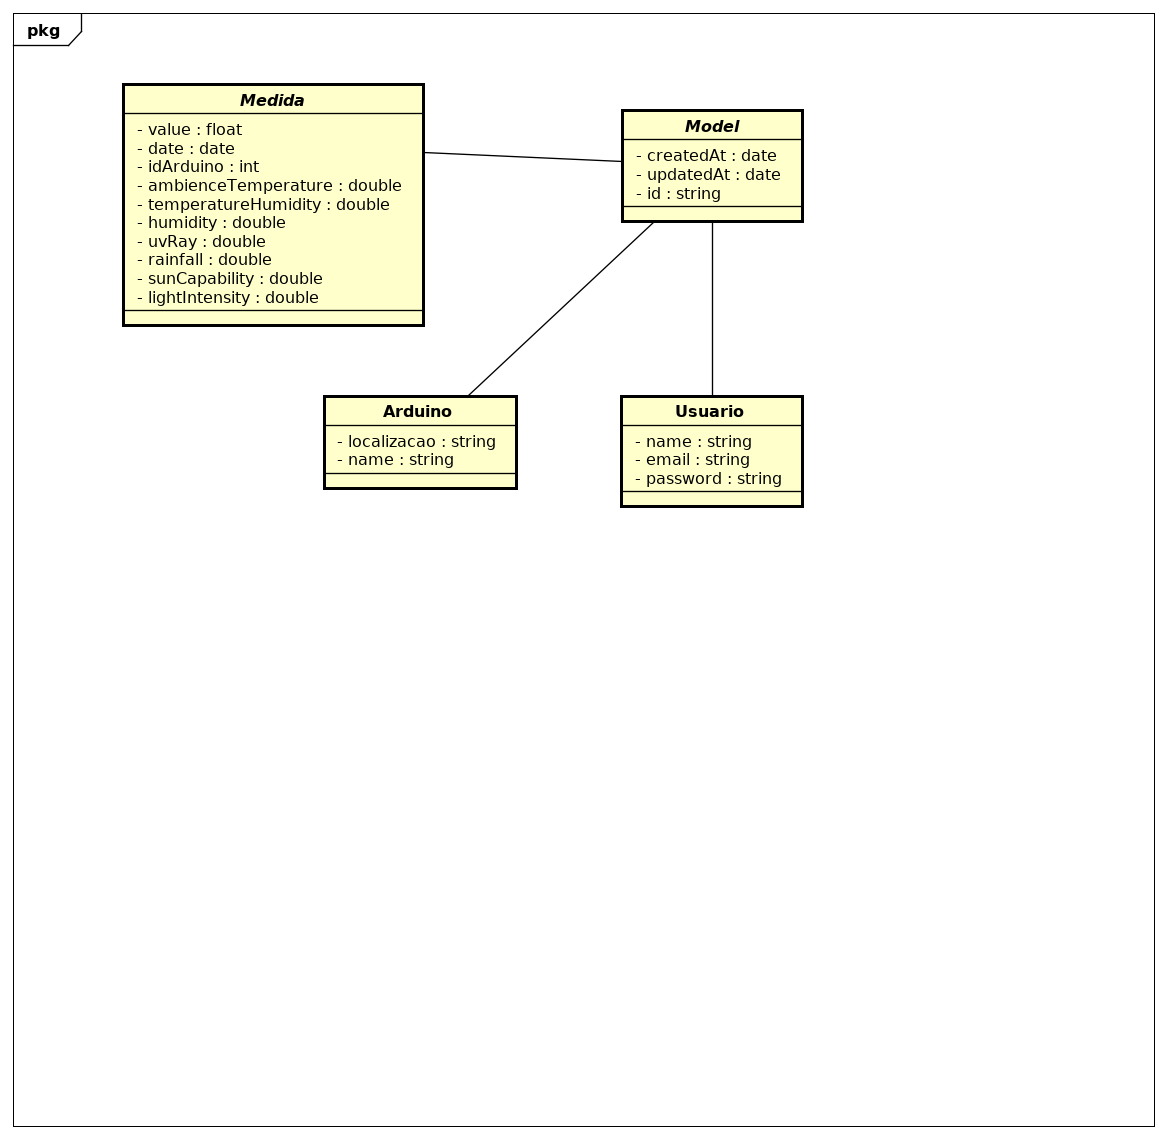
\includegraphics[scale=0.6]{diagrams/classe.png}
    \hfill
\end{figure}


\chapter{Diagrama de sequência}
\addcontentsline{toc}{chapter}{Diagrama de sequência}

Apresentação do diagrama de sequencia do projeto.

\begin{figure}[H]
    \label{figure_diagrama_sequencia}
    \centering
    \caption{Diagrama de sequência}
    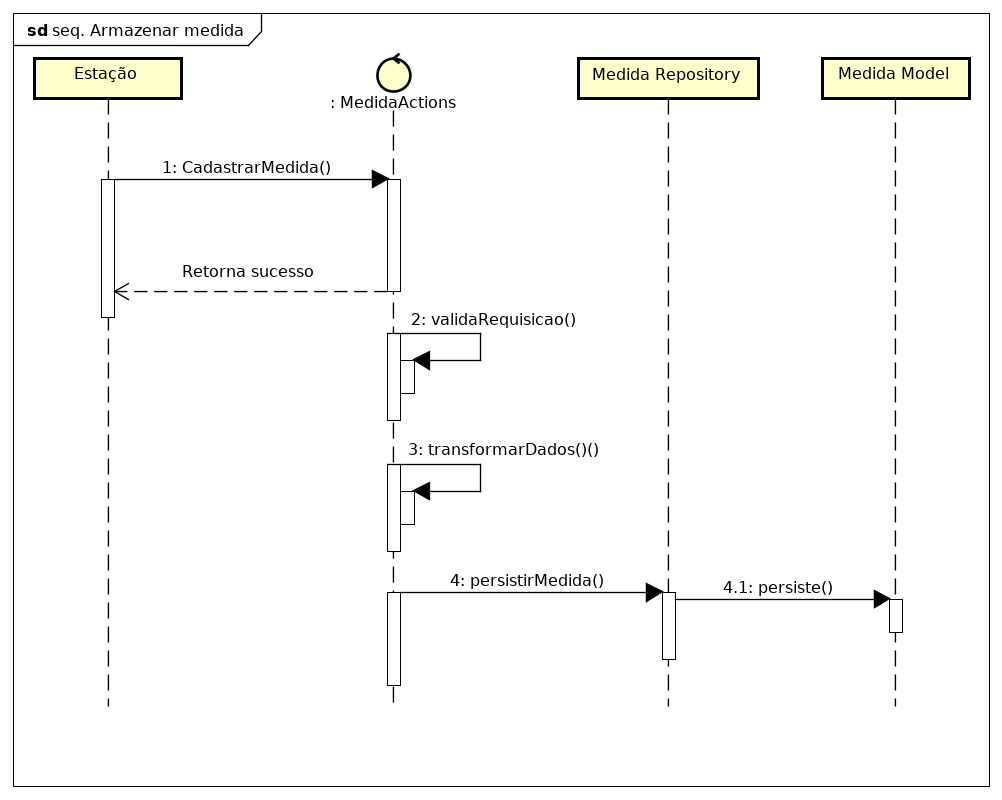
\includegraphics[scale=0.40]{diagrams/sequencia.png}
    \hfill
\end{figure}

Como descrito no diagrama de sequência representado na figura \ref{figure_diagrama_sequencia} a aplicação é composta por 3 principais camadas.

\section{Controlador}

Na camada de controle, os dados são recebidos e passam por uma básica validação através, porém não sofrem a interferência das regras de negócio.

Nessa camada, os dados são recebidos e retornados ao cliente, é uma interface de acesso a aplicação, geralmente, essa camada recebe objetos de requisições HTTP.

\section{Serviço de validação}

No serviço de validação, regras de negócio são aplicadas a medida para verificar se a mesma é valida para ser armazenada.

\section{Repositório}

Dentro da camada de repositório, são recebidos dados que, através de uma camada de infraestrutura são persistidos, retornando então, uma entidade.


\chapter{Diagrama de estado}
\addcontentsline{toc}{chapter}{Diagrama de estado}

Apresentação dos estados de uma entidade de medida que foi capturada ao longo da interação com o sistema.

\begin{figure}[H]
    \label{figure_diagrama_estado}
    \centering
    \caption{Diagrama de estado}
    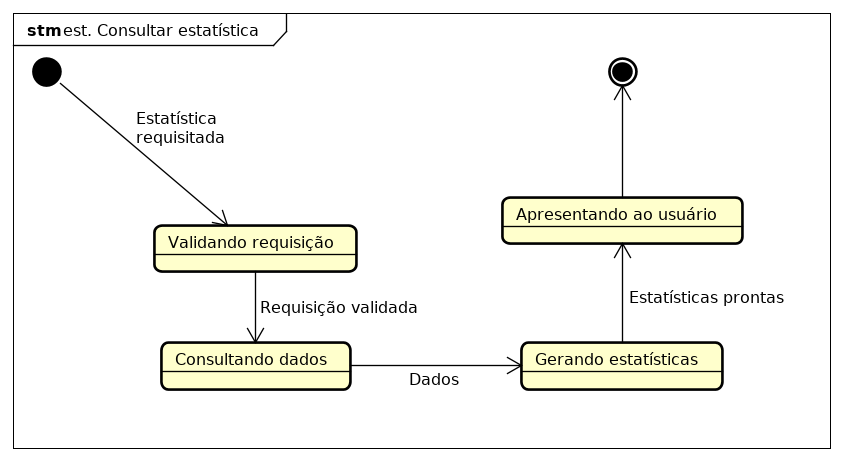
\includegraphics[scale=0.6]{diagrams/estado.png}
    \hfill
\end{figure}

Conforme descrito na figura \ref{figure_diagrama_estado} os estados durante o armazenamento de uma de uma medida são:

\section{Validando requisição}

A autenticação do arduino na API foi feita e a requisição HTTP para o armazenamento de uma medida foi feita até a API.
Nesse estado, a requisição está passando por uma validação básica, verificando os tipos e formato dos dados.

\section{Validando regras de negócio}

A medida passou pelo controlador e está sendo validada através dos filtros, onde as regras de negócio de validação estão verificando se aquela medida faz sentido, baseando-se nas medidas captadas anteriormente.

\section{Armazenando em banco de dados}

A medida é valida e está sendo armazenada no banco de dados, após, ela é retornada a camada de serviço.


\chapter{Diagrama de implementação}
\addcontentsline{toc}{chapter}{Diagrama de implementação}

A seguir o diagrama de implementação do sistema, que descreve a forma como os componentes de hardware e software interagem entre si.

\begin{figure}[H]
    \label{figure_diagrama_implementacao}
    \centering
    \caption{Diagrama de implementação}
    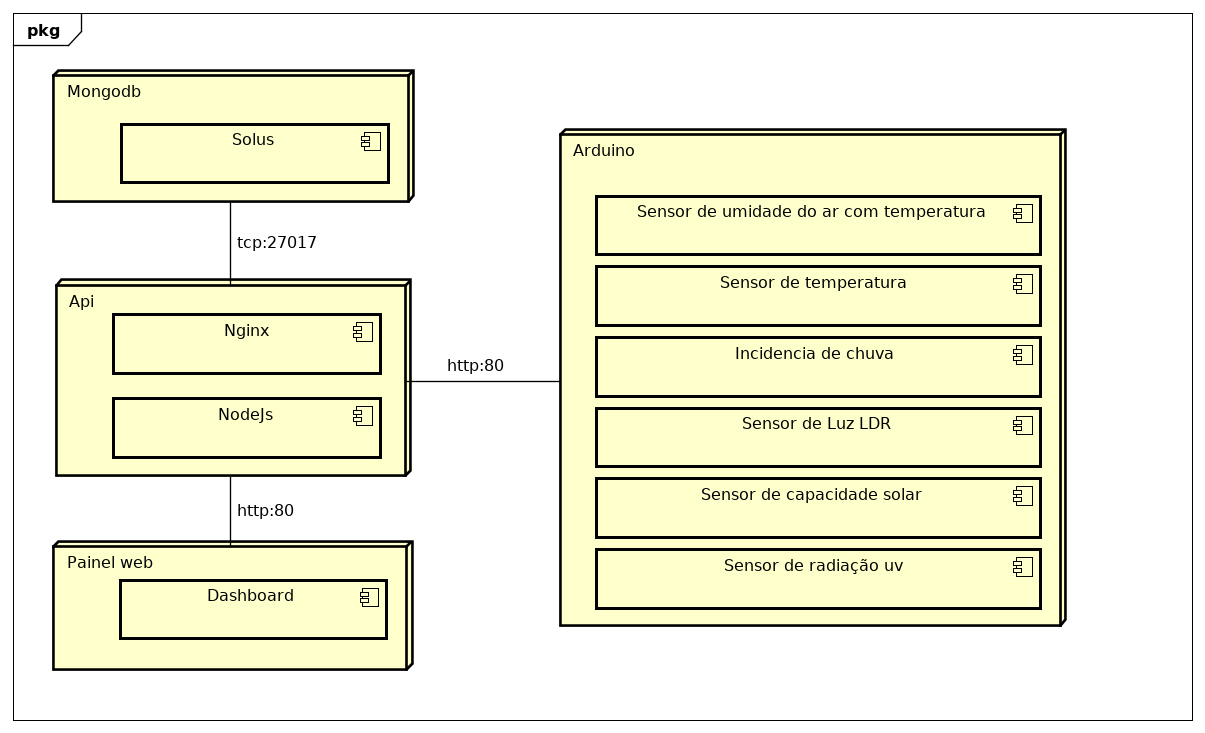
\includegraphics[scale=0.6]{diagrams/implementacao.png}
    \hfill
\end{figure}

\section{Sensores}

Os sensores do arduino, são ligados através da protoboard até o arduino, onde a captação é feita e as informações são tratadas, os dados são montados dentro de uma string JSON, que é enviada para o nodeMCU.

Não foi utilizada a biblioteca para a montagem da string JSON por conta da memória limitada do controlador.

\section{NodeMCU}

Na placa de WiFi NodeMCU, as informações são recebidas através da porta serial e o json recebido é enviado para a api.


\chapter{Descrição e arquitetura do banco de dados}
\addcontentsline{toc}{chapter}{Descrição e arquitetura do banco de dados}

O banco de dados utilizado foi o MongoDB, um banco de dados não relacional, o desenho do banco de dados é controlado pela aplicação, que define quis campos devem ser indexados e como os dados devem se "relacionar", cada informação capturada fica armazenada dentro de uma coleção, utilizando o formato JSON.

\section{Motivação}

A escolha de um banco de dados não relacional, foi motivada pela facilidade ao se trabalhar com esquemas maleaveis, podendo ter suas informações mutadas, deixando a cargo da aplicação a tomada de decisão.

O banco MongoDB foi escolhido pela sua facilidade ao trabalhar com escrita de dados concorrente, pois, as informações são, em primeiro instante processadas e armazenadas em cache, e já são retornadas para a aplicação, somente após, o MongoDB se encarrega de realizar a inserção dos dados em disco.

Com todas as vantagens do banco de dados, a aplicação tira vantagem, se beneficiando no que toca performance, disponibilidade e mutabilidade das informações.

\chapter{Descrição e documentação da API}
\addcontentsline{toc}{chapter}{Descrição e documentação da API}

Podemos conferir abaixo a documentação das rotas da API.

\begin{table}[H]
    \centering
    \caption{Descrição das rotas da API}
    \label{table_api_routes}
    \begin{tabular}{|l|l|l|}
    \hline
    \textbf{Método}  & \textbf{Rota}        & \textbf{Descrição}                           \\ \hline
    GET              & /arduino             & Lista os arduinos                            \\ \hline
    GET              & /arduino/:id         & Retorna os dados de um arduino               \\ \hline
    POST             & /arduino             & Cadastra um novo arduino                     \\ \hline
    POST, PATCH, PUT & /arduino/:id         & Atualiza os dados de um arduino              \\ \hline
    DELETE           & /arduino/:id         & Deleta um arduino e suas medidas capturadas  \\ \hline
    GET              & /user                & Lista os usuários                            \\ \hline
    GET              & /user/:id            & Retorna os dados de um usuário               \\ \hline
    POST             & /user                & Cadastra um novo usuário                     \\ \hline
    POST, PATCH, PUT & /user/:id            & Atualiza os dados de um usuário              \\ \hline
    DELETE           & /user/:id            & Deleta um usuário                            \\ \hline
    POST             & /user/login          & Recebe as credenciais e retorna o token      \\ \hline
    POST             & /measure             & Cadastra uma medida capturada                \\ \hline
    GET              & /statistic/:id       & Retorna as estatísticas de dados do arduino  \\ \hline
    \end{tabular}
\end{table}

\section{Métodos HTTP utilizados}

Como podemos visualizar na tabela \ref{table_api_routes}, o método POST fica designado a criar um recurso quando a requisição for enviada para uma rota sem a identificação. O método POST também é utilizado para atualizar um recurso quando a requisição for enviada para um recurso identificado. Para a atualização de um recurso também pode ser utilizado o método PATCH.
Para a consulta de recursos é utilizado o método GET, o método DELETE é utilizado para excluir um recurso.

\section{Autenticação}

A autenticação foi feita utilizando Json Web Token, onde, uma vez que o usuário tenha feito o login na API, as informações do usuário e seu token de acesso são retornados.

O token é passado para as rotas através dos cabeçalhos da requisição, onde a autenticação se faz necessária, o token enviado é validado, e caso seja invalido, o acesso ao usuário é negado.

% ----------------------------------------------------------
% Finaliza a parte no bookmark do PDF
% para que se inicie o bookmark na raiz
% e adiciona espaço de parte no Sumário
% ----------------------------------------------------------
\phantompart

% ---
% Conclusão
% ---
\chapter{Conclusão}
% ---

Conclusão



% --------------------------------
% ELEMENTOS PÓS-TEXTUAIS
% --------------------------------
% ----------------------------------------------------------
% ELEMENTOS PÓS-TEXTUAIS
% ----------------------------------------------------------
\postextual
% ----------------------------------------------------------

% ----------------------------------------------------------
% Referências bibliográficas
% ----------------------------------------------------------
\bibliography{references}

% ----------------------------------------------------------
% Glossário
% ----------------------------------------------------------
%
% Consulte o manual da classe abntex2 para orientações sobre o glossário.
%
%\glossary

% ----------------------------------------------------------
% Apêndices
% ----------------------------------------------------------

% ---
% Inicia os apêndices
% ---
%\begin{apendicesenv}
%
%% Imprime uma página indicando o início dos apêndices
%\partapendices
%
%% ----------------------------------------------------------
%\chapter{Quisque libero justo}
%% ----------------------------------------------------------
%
%\lipsum[50]
%
%% ----------------------------------------------------------
%\chapter{Nullam elementum urna vel imperdiet sodales elit ipsum pharetra ligula
%ac pretium ante justo a nulla curabitur tristique arcu eu metus}
%%
%
%\end{apendicesenv}
% ---


%---------------------------------------------------------------------
% INDICE REMISSIVO
%---------------------------------------------------------------------
\phantompart
\printindex
%---------------------------------------------------------------------


\end{document}
